% Created 2023-03-15 Wed 11:50
% Intended LaTeX compiler: pdflatex
\documentclass[a4paper]{article}
\usepackage[utf8]{inputenc}
\usepackage[T1]{fontenc}
\usepackage{graphicx}
\usepackage{longtable}
\usepackage{wrapfig}
\usepackage{rotating}
\usepackage[normalem]{ulem}
\usepackage{amsmath}
\usepackage{amssymb}
\usepackage{capt-of}
\usepackage{hyperref}
\usepackage{breakcites}
\usepackage{apacite}
\usepackage{paralist}
\usepackage{biblatex}
\addbibresource{/home/dp/Documents/Research_paper_SFR/bibl/bibliography/bibliography.bib}
\usepackage{hyperref}
\let\itemize\compactitem
\let\description\compactdesc
\let\enumerate\compactenum
\addbibresource{/bibl/bibliography/bibliography.bib}
\author{Dimitrios Papachistopoulos}
\date{\today}
\title{Finding the normalization constant of \(SFR_{del}\) and the relations between the various masses of the Galaxies}
\hypersetup{
 pdfauthor={Dimitrios Papachistopoulos},
 pdftitle={Finding the normalization constant of \(SFR_{del}\) and the relations between the various masses of the Galaxies},
 pdfkeywords={},
 pdfsubject={},
 pdfcreator={Emacs 28.2 (Org mode 9.6.1)}, 
 pdflang={English}}
\begin{document}

\maketitle
\tableofcontents

\#\#+\LaTeX{}\textsubscript{HEADER}: \affiliation{Dr. Pavel Kroupa}
\begin{ABSTRACT}


\textbf{Abstract}

\noindent\rule{\textwidth}{0.5pt}
\end{ABSTRACT}
\tableofcontents


\section{The Galaxies in the Local Cosmological Volume (LCV)}
\label{sec:org776cf02}

The Catalogue of Neigbouring Galaxies (Karachentsev, Igor D. and Makarov  et al. 2013\autocite{karachentsevUPDATEDNEARBYGALAXY2013}) and its updated version from the ``Catalog \& Atlas of the LV galaxies'' database \cite{CatalogLVGalaxies} are used to extract the K-band luminosities, the types of the galaxies, the mass within the Holmberg radius (M26), the Hydrogen masses of the galaxies (\(M_{HI}\)) and the SFRs based on integrated  H and far-ultraviolet (FUV) measurments for galaxies within a distance of
\(\approx 11\) Mpc. The SFR values contain limit flags, which we exclude from our present analysis. This gives a sample of 793 galaxies from 1248. From the remaing galaxies we have

\begin{center}
\begin{tabular}{|l|l|}
\hline
Measurment & Number of Galaxies \\
\hline
Hydrogen-Mass & 643 \\
M26 & 643 \\
K-band lum. & 789 \\
Type & 793 \\
H \$$\backslash$alpha\$ -S & 566 \\
FUV-SFR & 688 \\
\hline
\end{tabular}
\end{center}

The K-band values are converted to the total Stellar Masses of each galaxy according to the mass-to-light ratio of 0.6 (\cite{lelliSPARCMASSMODELS2016}), and the \(M_{HI}\) can be converted to the total mass of the gas of the galaxy using the equation \(M_g=1.33\,M_{HI}\)

The total SFR of each galaxy can be calcuated by

$$
    SFR_o=\frac{SFR_{FUV}+SFR_{Ha}}{2}
$$

if both \(SFR_{H\alpha},SFR_{FUV}\) measurments are available. If only one only one of them is given, then the SFR is equal to the given SFR value

$$
    SFR_o=SFR_i,\ \text{if } SFR_j=0,\ i\neq j,\ i,j=SFR_{FUV},\, SFR_{Ha}
$$

The condition \(SFR_o\geq 10^{-3}M_\odot yr^{-1}\) leaves 579 galaxies. This condition is applied due to the reasons given in the P. Kroupa,M. Haslbauer, I. Banik, S. T. Nagesh and J. Pflamm-Altenburg et al. 2020 \cite{kroupaConstraintsStarFormation2020}

\section{Types of galaxies}
\label{sec:org3f06310}

Using the dataset of 1248 galaxies, do before using the condition and removing the galaxies with the flags, the below histograms can be plotted.

\begin{figure}[htbp]
\centering
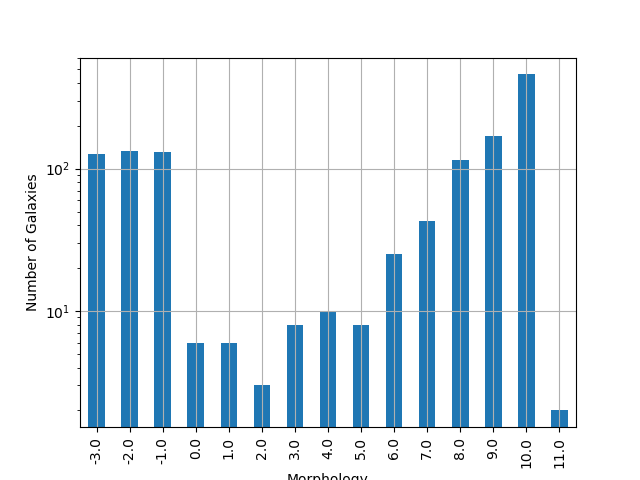
\includegraphics[width=.9\linewidth]{./graphs/hist-Type.png}
\caption{\label{Types of galaxies}The classification by de Vaucouleurs et al. (1991) is used for the morphology of the galaxies}
\end{figure}

Most of the galaxies in the LCV are Higly Irregular galaxies followed by lenticular galaxies

Out of the 1248 galaxies the 1022 are dwarf galaxies

\begin{figure}[htbp]
\centering
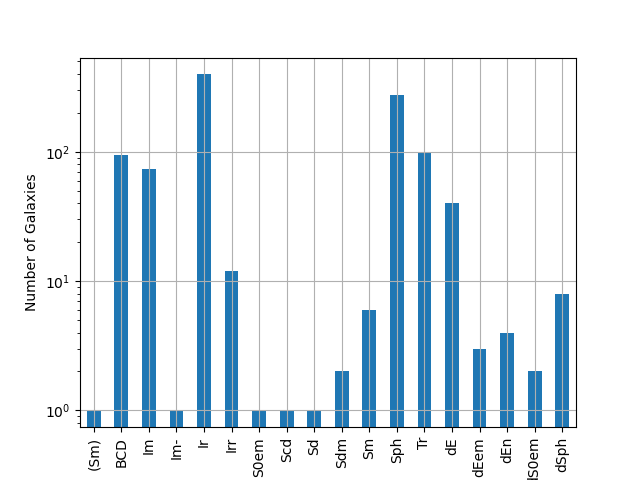
\includegraphics[width=.9\linewidth]{./graphs/hist-Tdw1.png}
\caption{\label{Types of dwarf galaxies}Dwarf galaxy morphology}
\end{figure}

\begin{figure}[htbp]
\centering
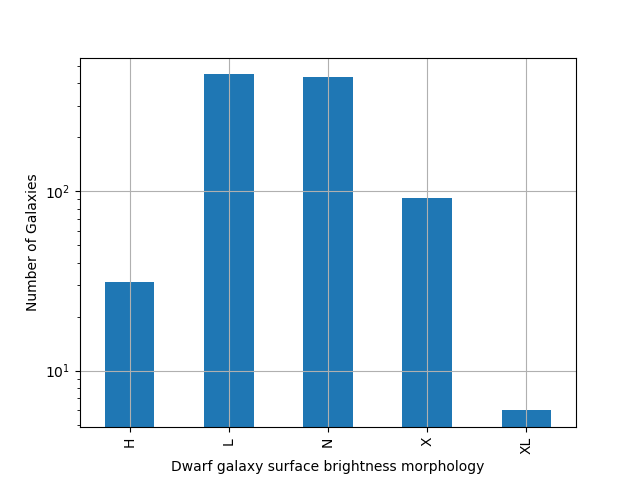
\includegraphics[width=.9\linewidth]{./graphs/hist-Tdw2.png}
\caption{\label{Types of dwarf galaxies brightness}Dwarf galaxy surface brightness morphology, where: H = high; N = normal; L = low; X = extremely low.}
\end{figure}

Most dwarf galaxies have low brightness and are irregulars followed by Dwarf spheroidal.

\section{Calculation of the normalization constant}
\label{sec:orgbfb382e}

According to P. Kroupa et al. 2020 current star formation rates of galaxies can be described by the 'delayed-\(\tau\)' mode as


\begin{equation} \label{eq:SFR}
SFR_{0,del}=\frac{A_{del}xe^{-x}}{\tau},\text{ where } x=\frac{t_{sf}}{\tau}
\end{equation}


\(\tau\) is the star formation time-scale and \(t_{sf}\) is the real time of star formation in a given galaxy

The average SFR is

\begin{equation}\label{eq:av_SFR-x}
\overline{SFR_{del}}=\frac{A_{del}}{t_{sf}}[1-(1+x)e^{-x}]
\end{equation}
and can also be defined by the present day stellar mass

\begin{equation}\label{eq:av_SFR M*}
    \overline{SFR}=\frac{\zeta M_*}{t_{sf}}
\end{equation}
where \(\zeta\) accommodates for mass-loss through stella evolution and \(\zeta\approx 1.3\)

\subsection{Constant \(t_{sf}\)}
\label{sec:org4bfffb4}
The observed ages of galactic discs are \(t_{sf}\approx 12\) Gyr (e.g. Knox, Hawkins \& Hambly 1999), so assuming an approximation of \(t_{sf}=12.5\) Gyr, the \(\overline{SFR_{del}}\) can be calcuated, from the equation (\ref{eq:av_SFR M*}). After that the equation of ratio


\begin{equation} \label{eq:ratio}
    \frac{\overline{SFR_{del}}}{SFR_{0,del}}=\frac{e^x-x-1}{x^2}
\end{equation}

can be solved numerically for \(x\) and using the equations (\Ref{eq:SFR}) and (\Ref{eq:av_SFR-x}) the \(A_{del}\) and \(\tau\) of each galaxy are found

\begin{verbatim}
                x           tau         A_del
count  550.000000  5.500000e+02  5.500000e+02
mean     1.762321  1.126908e+11  2.600301e+12
std      1.388768  1.067717e+12  4.456457e+13
min      0.000559  2.198306e+09  2.477977e+07
50%      1.513139  8.260984e+09  6.446495e+08
max      5.686198  2.237735e+13  1.005083e+15
\end{verbatim}

\begin{center}
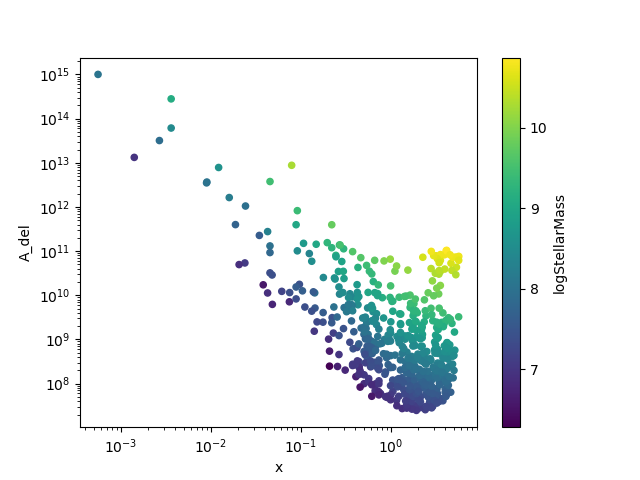
\includegraphics[width=.9\linewidth]{./graphs/x-A_3.png}
\end{center}

\subsection{Constant \(\tau\)}
\label{sec:org3e5bf87}
Assuming for an constant \(\tau=3.5\) Gyr, we cannot use the same \(\overline{SFR}\) and ratio. Using the equations\textasciitilde{}(\Ref{eq:av_SFR M*}) and (\Ref{eq:ratio})

$$
    \frac{\overline{SFR_{del}}}{SFR_{0,del}}=\frac{e^x-x-1}{x^2}\Leftrightarrow \frac{e^x-x-1}{x}=\frac{\zeta M_*}{SFR\cdot\tau}
$$

and \(x\) and \(A_{del}\) can be calcuated numerically.

\begin{verbatim}
                  A           tsf         x_i
count  5.500000e+02  5.500000e+02  550.000000
mean   4.192335e+09  8.727310e+09    2.493517
std    1.432226e+10  3.097809e+09    0.885088
min    9.870027e+06  2.323533e+09    0.663867
25%    6.466448e+07  6.441713e+09    1.840489
50%    2.234694e+08  8.383763e+09    2.395361
75%    1.034826e+09  1.077179e+10    3.077654
max    1.057699e+11  1.796414e+10    5.132611
\end{verbatim}


\begin{center}
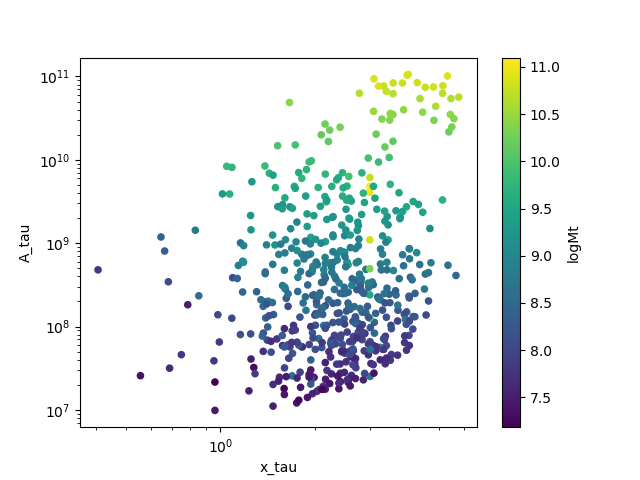
\includegraphics[width=.9\linewidth]{./graphs/x-A_tau.png}
\end{center}

Comparing the two different results for x, we see that the \(x_i\) from the second solution has a lower \(\sigma\)
\begin{verbatim}
                x         x_i
count  550.000000  550.000000
mean     1.762321    2.493517
std      1.388768    0.885088
min      0.000559    0.663867
25%      0.558532    1.840489
50%      1.513139    2.395361
75%      2.789068    3.077654
max      5.686198    5.132611
\end{verbatim}


The \(x_i\) results are more inline with the expected values from Kroupa et al. 2020 \(2.7<x<3.4\)
\begin{center}
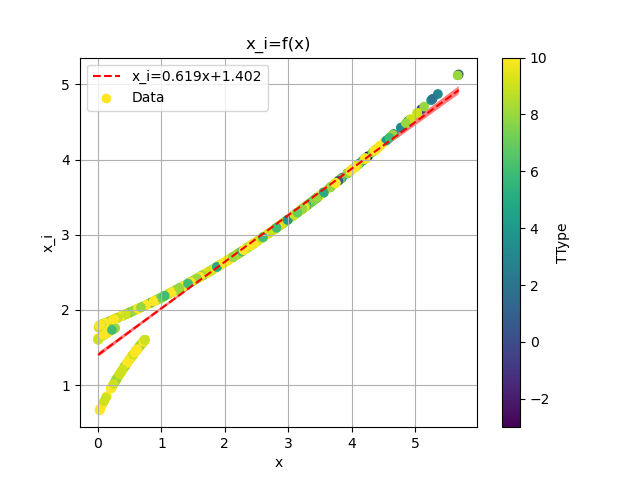
\includegraphics[width=.9\linewidth]{./graphs/x-x_i.png}
\end{center}

\begin{center}
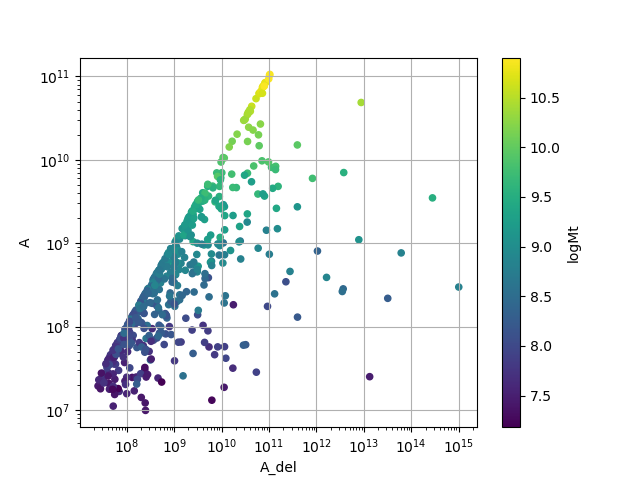
\includegraphics[width=.9\linewidth]{./graphs/A-A_del.png}
\end{center}

The correlation between the 2 different \(x\) is good with an R-squared of 94\%

\subsubsection{{\bfseries\sffamily TODO} DO sigma clipping for x to see if the x's are in agreement with the theoritical values}
\label{sec:org33fabf5}

\section{Mass relations}
\label{sec:orgcb5272f}

The below graphs show the correlation that the masses of the galaxies have. To consider a correlation good we need a \(R^2>70\%\)


\begin{figure}[htbp]
\centering
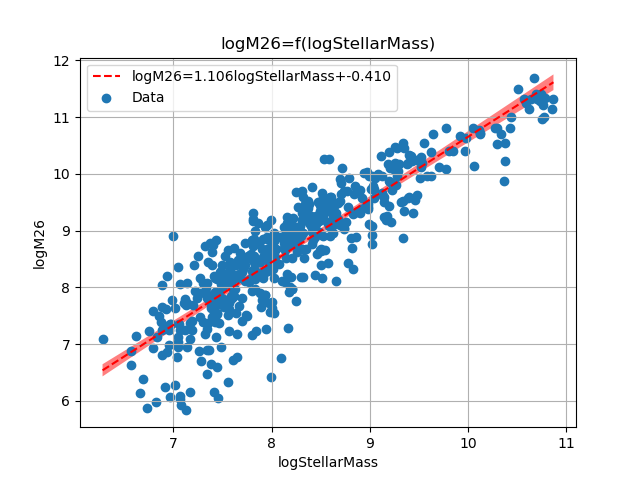
\includegraphics[width=.9\linewidth]{./graphs/logStellarMass-logM26.png}
\caption{\label{Stellar Mass - Mass within Holmberg radius}Stellar Mass - Mass within Holmberg radius: \(R^2=0.8\)}
\end{figure}


\begin{figure}[htbp]
\centering
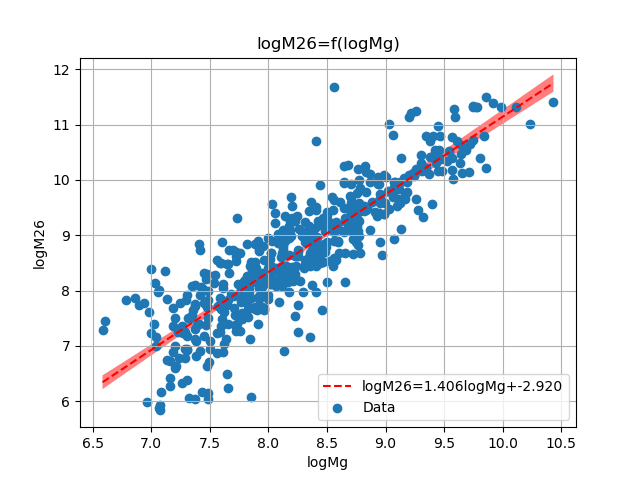
\includegraphics[width=.9\linewidth]{./graphs/logMg-logM26.png}
\caption{\label{Gas Mass - Mass within Holmberg radius}Gas Mass - Mass within Holmberg radius: \(R^2=0.77\)}
\end{figure}

\begin{figure}[htbp]
\centering
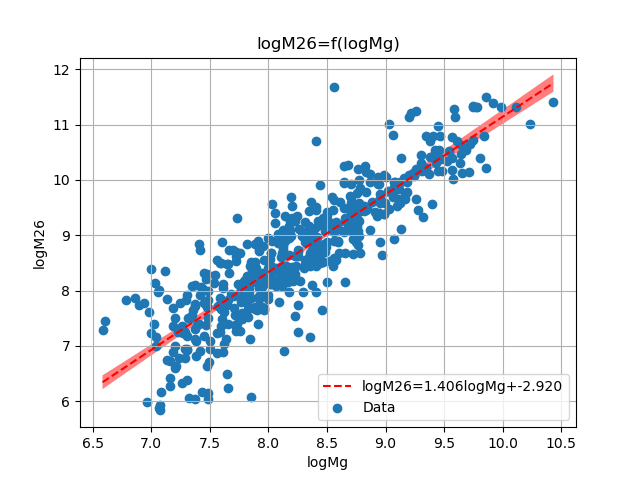
\includegraphics[width=.9\linewidth]{./graphs/logMg-logM26.png}
\caption{\label{Gas Mass - Mass within Holmberg radius}Gas Mass/Hydrogen Mass - Mass within Holmberg radius: \(R^2=0.77\)}
\end{figure}, \begin{figure}[htbp]
\centering
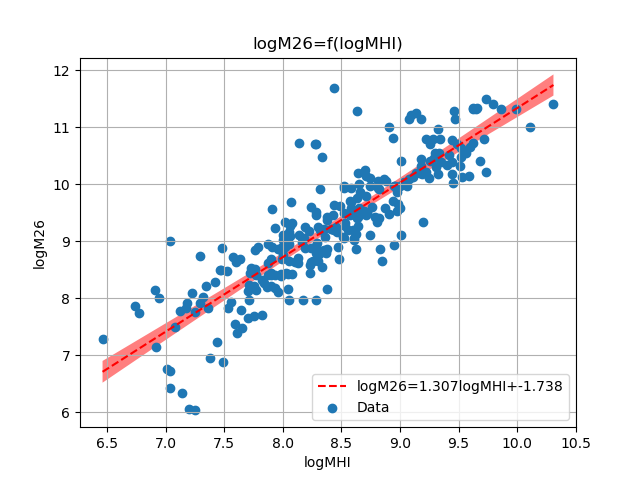
\includegraphics[width=.9\linewidth]{./graphs/logMHI-logM26.png}
\caption{\label{Gas Mass - Mass within Holmberg radius}Gas Mass/Hydrogen Mass - Mass within Holmberg radius: \(R^2=0.77\)}
\end{figure}

\begin{figure}[htbp]
\centering
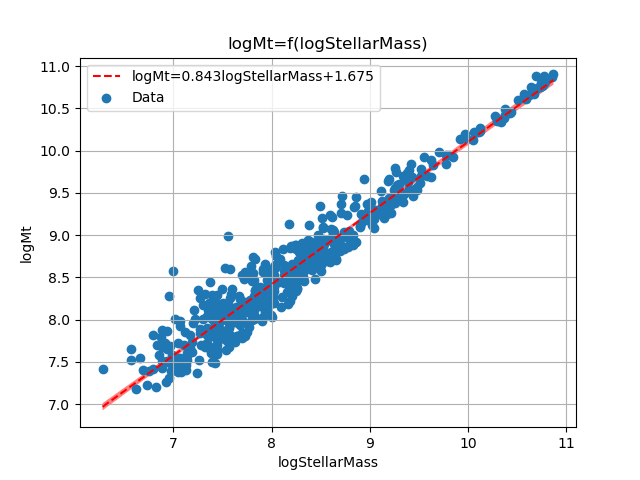
\includegraphics[width=.9\linewidth]{./graphs/logStellarMass-logMt.png}
\caption{\label{Total Mass - Stellar Mass}Total Mass - Stellar Mass: \(R^2=0.93\)}
\end{figure}

\begin{figure}[htbp]
\centering
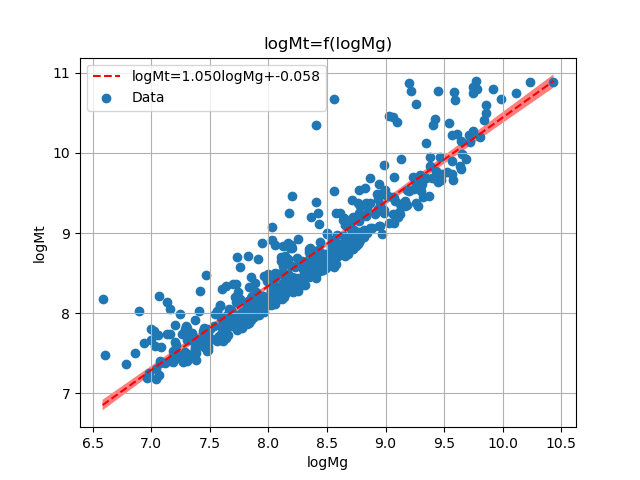
\includegraphics[width=.9\linewidth]{./graphs/logMg-logMt.png}
\caption{\label{Total Mass - Gas Mass}Total Mass - Gas Mass/Hydrogen Mass: \(R^2=0.87\)}
\end{figure},\begin{figure}[htbp]
\centering
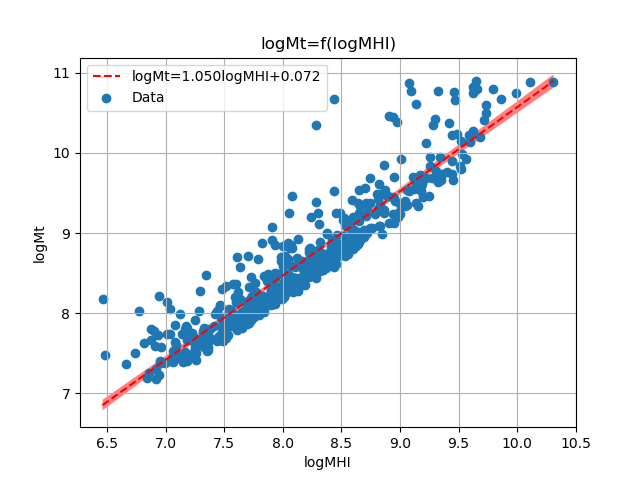
\includegraphics[width=.9\linewidth]{./graphs/logMHI-logMt.png}
\caption{\label{Total Mass - Gas Mass}Total Mass - Gas Mass/Hydrogen Mass: \(R^2=0.87\)}
\end{figure}

\begin{figure}[htbp]
\centering
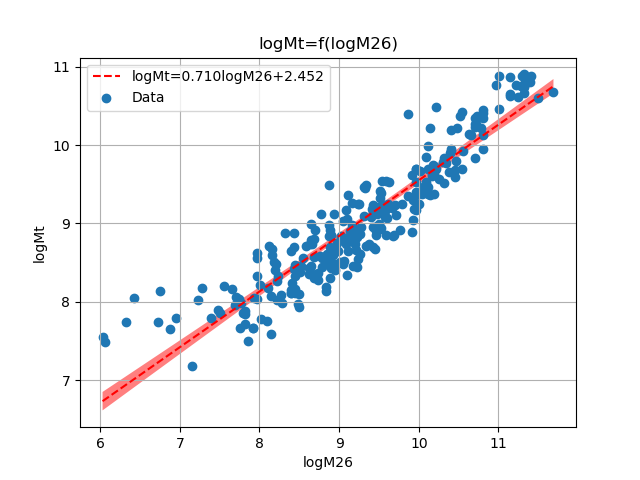
\includegraphics[width=.9\linewidth]{./graphs/logM26-logMt.png}
\caption{\label{Total Mass - Mass within Holmberg radius}Total Mass - Mass within Holmberg radius: \(R^2=0.85\)}
\end{figure}


\begin{figure}[htbp]
\centering
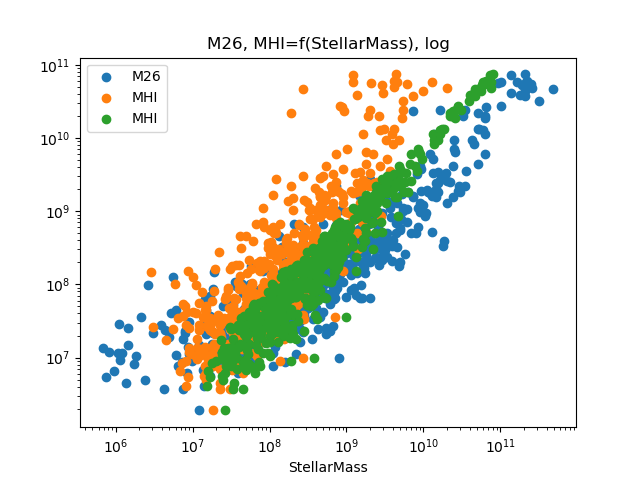
\includegraphics[width=.9\linewidth]{./graphs/M-MHI-M26.png}
\caption{\label{Stellar Mass - Mass within Holmberg radius - Hydrogen Mass - Total Mass}Stellar Mass - Mass within Holmberg radius - Hydrogen Mass - Total Mass}
\end{figure}


\section{Calculate the gas depletion timescale \(\tau_g\)}
\label{sec:orgf5cea8c}

The gas depletion timescale τg measures the time taken by a galaxy to exhaust its gas content Mg given the current SFR (Pflamm-Altenburg \& Kroupa 2009).
$$
\tau_g=\frac{M_g}{\dot{M_*}}=\frac{M_g}{SFR}
$$
\end{document}